\project{Functions and Mathematical Models}

\section{Purpose of this project}

An understanding of calculus can only be achieved if you, the student,
have a firm grasp on the concept of a function.  Literally everything
in this, and future, courses depends on it.  Therefore, in this
project we will explore what is meant by the term \textit{function},
and see how functions arise naturally in a number of application
areas.  Further, we will think about what a ``mathematical model'' is,
what they are used for, and the limits of their use.


\section{Background on Functions}
We recall from the class notes the following definition.

\begin{definition}
  A function $f$ is a rule giving a value, denote $f(x)$, for each
  $x$.  The set of $x$ for which $f$ is defined (i.e. for which the
  rule can be applied) is called the \emph{domain} of $f$, and the
  set of all possible values, $f(x)$, is called the \emph{range}.
  That is, the range of $f$ is the set
  \[
  \{f(x) \ | \ x \text{ is in the domain of $f$}\}.
  \]
\end{definition}

\bigskip

All of the functions encountered in math 221 will have a domain and
range that are \textit{subsets} of the real numbers.  Note that the
definition of a function is very broad and so particular functions can
be defined in a number of different ways as the next few examples
demonstrate.

\begin{example}
  Consider a vendor selling pizza by the slice on State Street.
  Suppose you can purchase 1, 2, 3, or 4 slices of pizza at a cost
  of \$2, \$3.75, \$5.25, and \$6.50, respectively.  The vendor
  does not take any other orders (that is, he will not allow you
  to purchase 5 slices since that is greedy).

  If we denote by $s$ the number of slices purchased, and by
  $p(s)$ the price of that order, in dollars, then $p$ is a
  function with domain $\{1, 2, 3, 4\}$ and range $\{2, 3.75,
  5.25, 6.50\}$.  The rule defining $p$ is then given by the
  following list
  \[
  p(1) = \$2, \quad p(2) = \$ 3.75,\quad p(3) = \$5.25, \quad p(4)
  = \$6.50.
  \]\hfill $\square$
\end{example}

\begin{example}
  A scientist at the Wisconsin Institute for Discovery believes that
  for every virus particle that infects a group of cells, one thousand
  new virus particles will be made.  If we let $v$ denote the number
  of virus particles that infect a group of cells, and by $f(v)$ the
  number of resulting virus particles, then $f(v)$ is a function with
  domain $\{0,1,2,\dots\}$ and range $\{0, 1000, 2000, \dots\}$
  defined by the rule
  \[
  f(v) = 1000\cdot v.
  \]
  Note that because the domain is no longer finite, it is no longer
  possible to give a list detailing the rule.\hfill $\square$
\end{example}

\begin{example}
  A car is moving away from you at a speed of 30 miles per hour.  At
  time zero, the car was already 2 miles away.  Let $t\ge 0$ denote
  time (in hours), and let $d(t)$ denote the distance between you and
  the car.  Then $d(t)$ is a function with domain $[0,\infty)$ and
  range $[2,\infty)$ defined by the rule
  \[
  d(t) = 2 + 30t
  \]\hfill $\square$
\end{example}

\vspace{.1in}

Of course, each of the functions above was derived from some (made up)
``real world'' application.  In a math course we will typically
consider functions with no overt connection to the ``real world.''
For example, as in the class notes on page 9, we can define $f(x)$ to
be the function defined piecewise via
\[
f(x) = \left\{\begin{array}{cc}
  2x & \text{ for } x < 0\\
  x^2 & \text{ for } x \ge 0
\end{array}\right..
\]
Having such flexibility allows us to play with an infinite number of
examples.

\subsection{Functions and Mathematical models}

A \textit{mathematical model} is a mathematical description of some
real world phenomenon.  Usually the model is described via an equation
or a system of equations.  The purpose of a mathematical model is to
gain insight into the phenomenon being studied and, hopefully, to make
predictions.

\begin{example}\label{example:manufacture}
  Consider a large manufacturer of Bucky Badger shirts.  Every year,
  the company spends \$200,000 on fixed operational costs (wages,
  electricity, mortgage, etc.).  Further, every shirt made costs an
  addition \$5.  Let $q$ denote the number of shirts produced by the
  company in a given year, and let $C(q)$ denote the cost to
  manufacture $q$ shirts.  Assume that if zero shirts are ever
  produced, they will fire all their employees and close their factory
  yielding a manufacturing cost of zero.\hfill$\square$

\end{example}

\section{Problems}
\problemfont
\problem What is the domain of the function $C$?  What is the range?

\problem A quantity of great interest to many manufacturers is the
\textit{marginal cost}, defined as the cost required to produce one
addition unit.  That is, the marginal cost at 5 units is the
difference in the cost of 6 and 5 units.  Define a function giving the
marginal cost for our manufacturer.  Be clear in specifying a domain,
range, and rule.

\problem Our manufacturer does not only care about costs, but also
wants to know about revenue.  Suppose they sell each unit for \$13.
Write down a function for revenue, $R(q)$, generated by selling the
Bucky Badger shirts, being careful to specify an appropriate domain
and range. How many shirts would need to be sold to make it worthwhile
to manufacture them?  Be explicit in how you solved this problem.  A
graph would certainly help.
\noproblemfont


\section{Relative risk and the effects of exercise on rates of breast
cancer}
\label{example:cancer}
According to the Susan G. Komen foundation for the
Cure\footnote{See,
\url{http://ww5.komen.org/BreastCancer/UnderstandingRisk.html}},
we define the \textit{absolute risk} as a person's chance of
developing a certain disease over a certain period of time.  Next, a
\textit{relative risk} is calculated by comparing two absolute
risks. The numerator (the top number in a fraction) is the absolute
risk among those with the risk factor. The denominator (the bottom
number) is the absolute risk among those without the risk factor.
Hence,
\[
\text{Relative risk} = \frac{\text{Absolute risk with
factor}}{\text{Absolute risk without factor}}.
\]

Note therefore, that if the relative risk of an activity is above
1.0, then the risk is higher for those people performing that
activity.  If, on the other hand, the relative risk is below 1.0,
then the risk is lower for the portion of the population performing
that activity is lower than the population at large.\vspace{.2in}

We present the following case study, that is based on a similar
study performed in Duke University's Laboratory Calculus course.
For reference, the data used in this study is taken from a study of
women, age 50 - 64, that were residents of King County in
northwestern Washington State.\footnote{\textit{Occurrence of Breast
Cancer in Relation to Recreational Exercise in Women Age 50 - 64
Years}, Epidemiology, Nov. 1996, Vol. 7, No. 6, 598 - 604}

\vspace{.2in}

One risk factor considered in the King County study was exercise
level.  The researchers asked each participant in the study ``During
the 2-year period prior to (date of study), with what frequency did
you do any strenuous physical activities, exercise, or sports?''
The following data was collected:
\begin{center}
  \begin{tabular}{lcccc}\toprule
    Average number of exercise hours per week & 0 & 2.0 & 3.0 & 4.0\\
    \midrule
    Relative Risk & 1.07 & 0.79 & 0.73 & 0.65 \\ \bottomrule
  \end{tabular}
\end{center}
This data in the table above is plotted in Figure \ref{fig:exercise}
\begin{figure}
  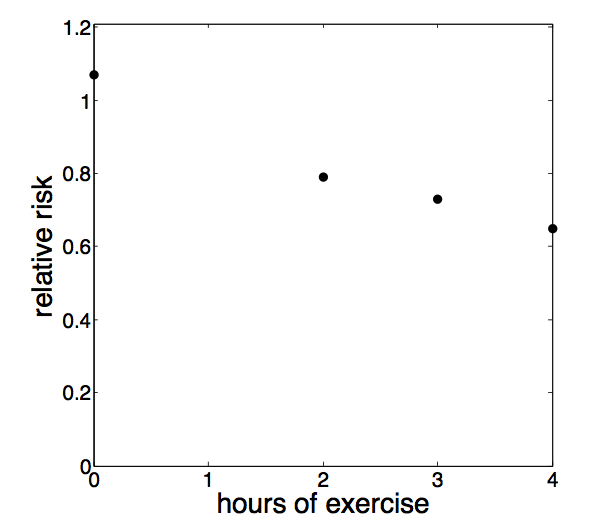
\includegraphics[scale=0.6]{Project1_ExVsRR.png}
  \caption{Relative risk of breast cancer vs. hours of exercise.}
  \label{fig:exercise}
\end{figure}

\section{Problems}
\problemfont
\problem
\subprob  Draw a straight line in Figure \ref{fig:exercise} that fits
the data well (do not use the statistical features of your
calculator).  Denote the relative risk by the variable $R$, and
hours of exercise by the variable $E$.  Determine the slope of the
line you drew.  Also determine the $R$ intercept.  What is the
equation of the line?

\subprob  What does the $R$ intercept tell you about exercise and the
relative risk of breast cancer?  is your intercept the same as
your data point on the axis?  Which do you think is more accurate?
Why?

\subprob  The slope of your line should be negative.  Describe what this
means in terms of relative risk of breast cancer and exercise.

\subprob  What is the absolute value of the slope?  Use this number and
the negativity of the slope of the line to finish the following
sentence: ``If a woman increases her exercise by one hour per
week, then her relative risk of breast cancer will be
(approximately) ....''

\subprob  Estimate the relative risk of breast cancer if a woman
exercises for 3.3 hours per week.

\subprob  Find the $E$ intercept (the place where the line intersects
the horizontal axis), and denote it by $M$.  Interpret $M$.

\subprob  For what values of $E$ do you believe your linear model to be
a decent approximation to the true relative risk?
\noproblemfont

\section*{Report Instructions}
Using complete sentences (including punctuation!), write out your
solutions to the exercises found in Example \ref{example:manufacture}.
Next, carefully write up your answers to the questions found in
Example \ref{example:cancer}.  You should include not only the
formulas used, but also all the derivations of the formulas.  General
instructions:
\begin{enumerate}
\item Do not turn in your first draft.  Instead, solve all the
  problems first, and then write or type up a clean report.
\item Only one report is required per group, but all members must take
  an active role in the solution and writing of the report.  If a
  member does not participate, his or her name should not be included
  on the final report.
\end{enumerate}

